 %
% File acl2018.tex
%
%% Based on the style files for ACL-2017, with some changes, which were, in turn,
%% Based on the style files for ACL-2015, with some improvements
%%  taken from the NAACL-2016 style
%% Based on the style files for ACL-2014, which were, in turn,
%% based on ACL-2013, ACL-2012, ACL-2011, ACL-2010, ACL-IJCNLP-2009,
%% EACL-2009, IJCNLP-2008...
%% Based on the style files for EACL 2006 by 
%%e.agirre@ehu.es or Sergi.Balari@uab.es
%% and that of ACL 08 by Joakim Nivre and Noah Smith

\documentclass[11pt,a4paper]{article}
\usepackage[hyperref]{acl2018}
\usepackage{times}
\usepackage{latexsym}
\usepackage{booktabs}
\usepackage{url}
\usepackage{amsmath}	% for \begin{align}
\usepackage{graphicx}	% for \includegraphics{filename}
\usepackage{subcaption}	% for \begin{subfigure}[t]{0.5\textwidth}
\usepackage{courier}	% for \texttt{}

\aclfinalcopy % Uncomment this line for the final submission
%\def\aclpaperid{***} %  Enter the acl Paper ID here

%\setlength\titlebox{5cm}
% You can expand the titlebox if you need extra space
% to show all the authors. Please do not make the titlebox
% smaller than 5cm (the original size); we will check this
% in the camera-ready version and ask you to change it back.

\newcommand\BibTeX{B{\sc ib}\TeX}

\title{Improving Sequence-to-Sequence with Adaptive Beam Search \newline \newline	
		Assignment 1}

\author{Yu-Hsiang Lin \quad Shuxin Lin \quad Hai Pham \\
  Language Technologies Institute \\
  Carnegie Mellon University \\
%   Affiliation / Address line 3 \\
{\tt\small $\left\{yuhsianl, shuxinl, htpham\right\}$@andrew.cmu.edu}
%   {\tt email@domain} 
%   \\\And
%   Second Author \\
%   Affiliation / Address line 1 \\
%   Affiliation / Address line 2 \\
%   Affiliation / Address line 3 \\
%   {\tt email@domain} \\
  }

\date{}

\begin{document}
\maketitle
\begin{abstract}
We plan to apply new techniques such as combining dynamical beam size with trainable beam search to boost up the training and test-time decoding of the sequence-to-sequence model. We review the related approaches, and report the preliminary experiment setting and results.
\end{abstract}

%%%%%%%%%%%%%%%%%%%%%%%%%%%%%%%%%
%         INTRODUCTION              
%%%%%%%%%%%%%%%%%%%%%%%%%%%%%%%%%
\section{Introduction} \label{sec:introduction}
Since its invention, sequence-to-sequence (seq2seq) model \cite{seq2seq_2014} has been a go-to model for many translation-related tasks,  % probably more examples needed 
especially since the advent of attention model \cite{bahdanau2014neural,luong2015effective}. Despite its great successes in many domains, how to train and decode seq2seq model is still an open problem because of the drawback of traditional maximum likelihood training which is, most of the cases, unable to find the maximum-a-posteriori of a to-be-decoded single sentence over the whole corpus. 

Amongst many heuristic approaches to remediate that problem, \textit{greedy search} and \textit{beam search} are probably the most popular. While greedy search is known for its lightweight, elegant characteristics, beam search is generally better in practice by considering not only the best-scored word at each time step but maintaining a window of best words. 
In this project, we will be addressing the disadvantages of previous approaches for seq2seq using beam search and proposing an improvement for it in training and decoding phases. We also present our results on the Name Entity Recognition task.

%%%%%%%%%%%%%%%%%%%%%%%%%%%%%%%%%
%         RELATED WORK              
%%%%%%%%%%%%%%%%%%%%%%%%%%%%%%%%%
\section{Related Work} \label{sec:related_work}% Literature Review 
The straightforward approach to improve seq2seq model trained with the traditional maximum likelihood method  of ground truths is to improve the decoding phase. While beam search is considered the de-factor approach \cite{seq2seq_2014}, greedy search, if designed properly, can yield a comparable performance, if not better in some cases, while having a much more lightweight architecture. \citet{goyal2017differentiable} proposed an approximated version of greedy search over the scheduled sampling training procedure \cite{bengio2015scheduled}. 
%% PROBABLY NEED MORE REFERENCE for REINFORCE
% Reinforcement learning 
Unlike tackling with decoding phase solely, another useful approach to improve seq2seq is to design a better architecture or technique of helping decode right on the training phase. One widely-employed approach is to 
%is to avoid the low performance of greedy search and high delay of beam search, 
convert it into an imitation learning problem \cite{daume2009search,ross2011reduction,bengio2015scheduled} where expert guidance from human is injected to make the agent more robust and efficient. 
A naturally connected method is to use reinforcement learning \cite{sutton1998reinforcement} which employs a reward-based loss instead of maximum likelihood-based \cite{ranzato2015sequence, gu2017learning}, giving rise to a new family of techniques which is fitted to the discrete text domain. 

% Reinforcement learning
While discriminative training is the straightforward method for seq2seq training, another generalized method is to pose it as a generative model. Amongst such solutions, Generative Adversarial Network \cite{goodfellow2014generative} broadly used for diverse tasks, predominantly in generating images \cite{dcgan2015,berthelot2017began,zhang2017stackgan,progressive_gan_2017,li2017mmd} and videos \cite{vondrick2016generating} based on what model learned from training, or \textit{translating} them given a style of images \cite{conditional_gan_2014,pix2pix2017,discoGAN2017,mechrez2017photorealistic,luan2017deep,zhu2017unpaired,ma2018gan} and videos \cite{ruder2016artistic,liu2017unsupervised}. Despite the booming trend of GAN, its application to text domain faces a difficult obstacle of inherent discrete properties of text domain. Nonetheless, there have been successes of translating text from a style to another 
%using professor-forcing \cite{professor_forcing_2016} 
to deal with discrete texts \cite{boundaryseeking_gan_2017,yu2017seqgan,shen2017style}.  
Another workaround when facing discrete text in designing a generative model is to use variational autoencoder \cite{kingma2013auto} with maximum likelihood objective to learn the disentangled latent representations into some controlled attributes \cite{controlled_text_gen_2017}. 

Inspired by GAN's design, similar approaches have been made to seq2seq in conjunction with reinforcement learning \cite{kusner2016gans, yu2017seqgan,gu2017neural, gumbel2017}. And although not directly connected, actor-critic setting which shares a close equivalence with GAN \cite{pfau2016connecting}, has been also employed to replace maximum-likelihood method \cite{bahdanau2017actor}. And while sharing the same methodology in that we improve the decoding performance by making the model learn to decode right on the training phase, our approach still sticks to maximum likelihood method objective for its straightforwardness and more simplicity in its design.  

%%% TODO: discrete search-based 
While reinforcement learning can yield a fast decoding model, training with maximum likelihood has its own merit of being simple yet comparably efficient. For such approach, some attempts to make the model learn how to decode right on the training phase have also taken place. There were some solutions that optimize beam search in discrete space such as from \citet{wiseman2016sequence, andor2016globally} whose target is to get rid of label bias problem and design a model that is globally--rather than locally--normalized. Another work, from which our work extends, instead aims at design a new surrogate training objective to convert from discrete space into a continuous approximation of the beam search \cite{goyal2018continuous}. In detail, because using beam search right at training phase largely degrades the performance due to its resources consumption and its search space, we plan to use a tactic of dynamic beam search \cite{buckman2016transition} to make the training faster while retaining its efficacy. 
% Our work instead tackles with the training phase rather than only looking at improving decoding. 

% Other more efficient seq2seq improvement approach is to address the disadvantages of maximum likelihood training and so change the target objective.

%%%%%%%%%%%%%%%%%%%%%%%%%%%%%%%%%
%           MODEL
%%%%%%%%%%%%%%%%%%%%%%%%%%%%%%%%%

\section{Model} \label{ssec:model}

The seq2seq model we use for this assignment is based on the encoder-decoder structure. Figure \ref{fig:fig_architecture} shows the model architecture.

\subsection{Encoder}

The encoder and decoder each consists of a single-layer long short-term memory (LSTM) network. The input sequence $X = \{x_1, x_2, \dots, x_{T_x}\}$ is first fed into an embedding layer $E^x$, and the resulting embeddings of $X$ are then feed into the encoding LSTM. The initial cell and hidden states are set as
\begin{align}
	\overrightarrow{c}_0 = 0, \\
	%
	\overrightarrow{h}_0 = 0,
\end{align}
respectively.

%%%%%%%%%%%%%%%%%%%%%%%%%
\begin{figure}[h]
\centering
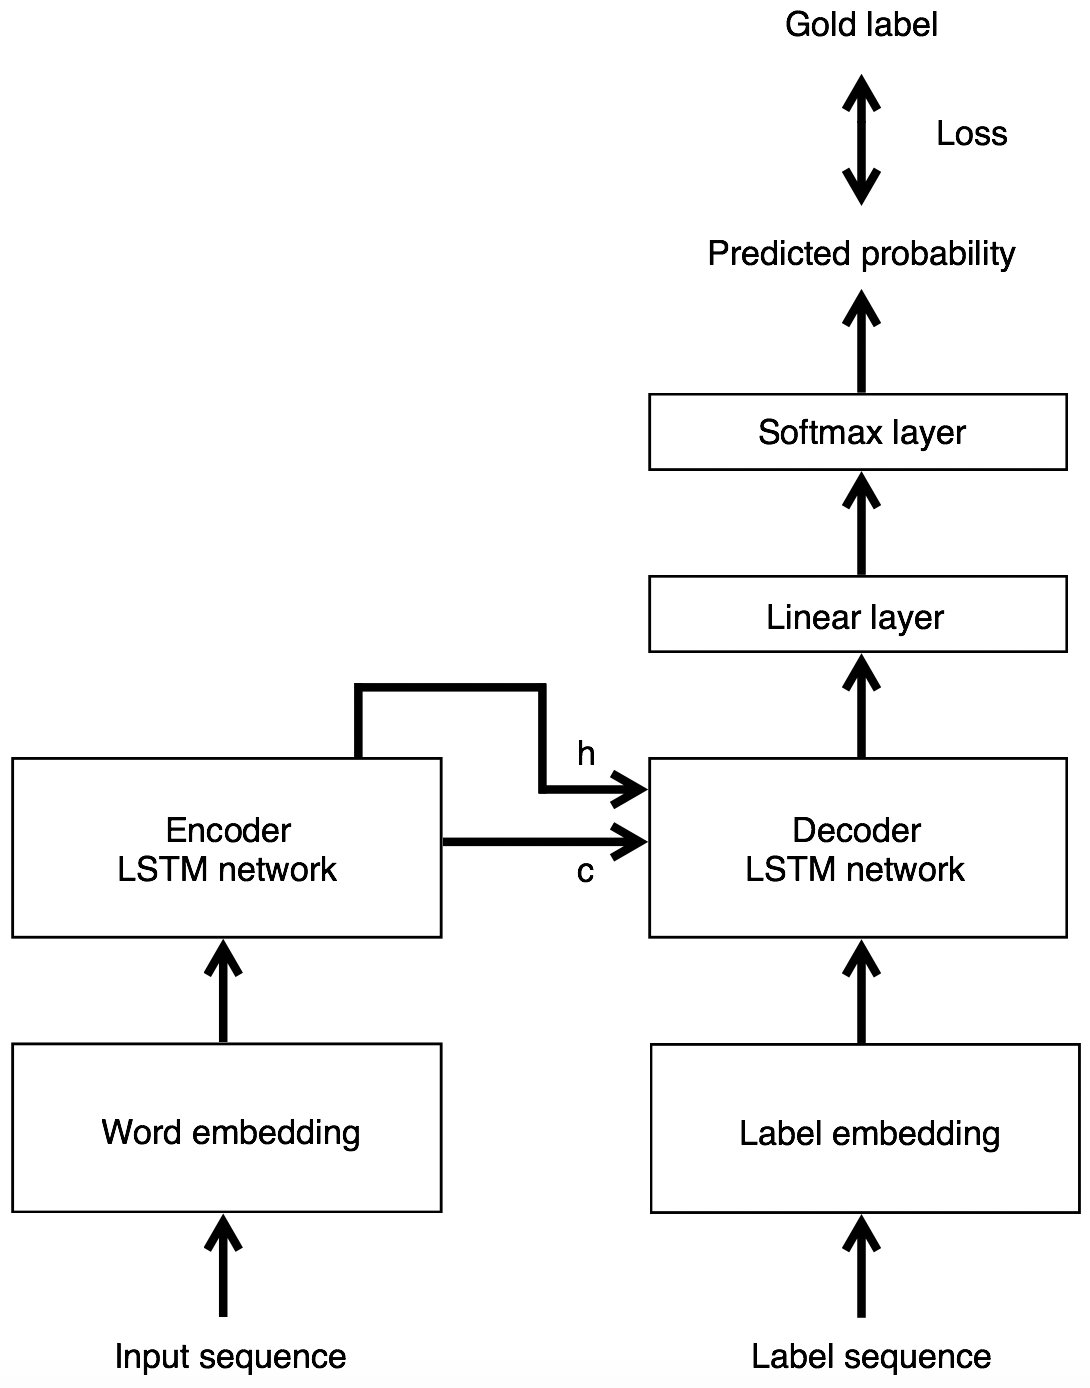
\includegraphics[width=0.8\linewidth]{fig_architecture}
\caption{The architecture of the neural seq2seq model.}
\label{fig:fig_architecture}
\end{figure}


\subsection{Training-time decoding}

In training time, the decoder receives the last hidden and cell states from the encoder as the initial hidden and cell states, respectively:
\begin{align}
	h_0 &= \overrightarrow{h}_{T_x}, \\
	%
	c_0 &= \overrightarrow{c}_{T_x}.
\end{align}
The golden label sequence $Y = \{y_1, y_2, \dots, y_{T_y}\}$ is also first casted into an embedding created by the target-space embedding layer $E^y$, and then fed into the decoding LSTM network. Note that, slightly different from the encoder, here it is $y_{t-1}$ that is fed into the LSTM cell at step $t$ (hence actually the last label $y_{T_y}$ is not fed as the input of the decoder; the input sequence is $\{y_0, y_1, \dots, y_{T_y - 1}\}$). For the initial input at step $t = 1$, we use an universal $y_0 = y_0^*$ to denote the beginning of the label sequence.

The hidden states $h_t$ is then fed into a linear layer to produce the score vector $s_t$, where each element of $s_t$ is the score for each of the possible labels at step $t$:
\begin{align}
	s_t = W_s h_t + b_s.
\end{align}
We then take the softmax over the score vector $s_t$ to obtain the probabilities of all possible labels at step $t$,
\begin{align}
	\label{eq:pt} p_t = \textrm{softmax}(s_t).
\end{align}

The loss at step $t$ is the cross entropy between the prediction $p_t$ and the golden label $y_t$,
\begin{align}
	L_t = -\log (p_t)_{y_t}.
\end{align}
The total loss for this sequence instance is the average of the loss over the steps,
\begin{align}
	L = \frac{1}{T_y} \sum_t L_t.
\end{align}
We take average in hope to remove the bias introduced by the length of the sequence.



\subsection{Test-time decoding}

In test time, as in training time, the decoder receives the last hidden and cell states from the encoder as the initial hidden and cell states. The initial input at step $t = 1$ is also the universal $y_0 = y_0^*$. Different from training time, the inputs at time $t = 2, \dots, T_y - 1$ depend on the predicted label at the previous step. Roughly speaking, we would ``replace'' the input $y_{t-1}$ in training time by $\hat{y}_{t-1}$ at test time. The exact way to do so is determined by the decoding algorithm.

In this assignment, we use the greedy decoding (beam search with fixed beam width 1) at test time. At step $t = 1$, we compute $p_1$ using \eqref{eq:pt}, and pick element $\hat{y}_1$ who has the highest probability $p_1$ as our predicted label. We keep an accumulated probability $P_t$ initialized as $P_1 = p_1$. At step $t = 2, 3, \dots, T_y$, after computing $p_t$, we first compute the accumulated probability $P_t = p_t P_{t-1}$, and then pick element $\hat{y}_t$ who has the highest probability $P_t$ as our predicted label at step $t$.



%%%%%%%%%%%%%%%%%%%%%%%%%%%%%%%%%
%         EXPERIMENT              
%%%%%%%%%%%%%%%%%%%%%%%%%%%%%%%%%
\section{Experiment}

Our implementation\footnote{The Github repository can be accessed at: https://github.com/ShuxinLin/nn4nlp\_project/.} is built based on PyTorch \cite{paszke2017automatic}. We conducted all experiments on AWS EC2. As it is discussed in Section \ref{ssec:model}, the current seq2seq model is the encoder-decoder architecture, with the encoder and decoder each consisting of an one-layer LSTM. We perform the experiments using mini-batch training and stochastic gradient descent (SGD) optimizer on a common natural language processing task, the named entity recognition (NER). The purpose of this project is to evaluate the effectiveness of our improvement to the seq2seq models, so we choose NER as our task even though the encoder-decoder model may not be the most suitable model for this task.


\subsection{Named Entity Recognition} \label{ssec:ner}

For named entity recognition, we use the data of CONLL-2003 shared task \cite{tjongkimsang2003conll} for English and German language. The data consists of three files per language: one training file and two test files, testa and testb. We use testa as the development data, testb as the final test data. In the current development phase, only the train data and the development data are used for finding good parameters for the seq2seq model. 

We perform minimum preprocessing on the data, since the best performance is not our ultimate goal of this project, but the effectiveness of the improvement we propose. The label has 9 possible values: 8 NER tags and a tag denoting the end of the sentence (EOS).


\subsection{Parameter Tuning} \label{ssec:paratune}

Before we start to experiment on the new search algorithms to improve the training and decoding of the seq2seq model, we first explore the effect of the choices of the hyperparameters on the performance of the neural networks. The hyperparameters we investigate are the batch size, the learning rate, the dimension of the word embeddings, and the number of the hidden units of the encoder. Once the parameter tuning is done, we plan to use pre-trained model for transfer learning and further fine tuning.


\subsection{Result} \label{ssec:baseline}
% detail of setup e.g. OpenNMT, PyTorch, hyper params etc 
Currently we conducted 5 experiments on the NER tasks. The basic model has hyperparameter settings of $batch\_size=16$, $learning\_rate = 0.1$, $dim\_word\_embed =100$, and $hidden\_units=64$. For each experiments, we run 300 iterations due to the limited time. Figure \ref{fig:fig_exp1} shows the cross-entropy loss of the training data of the NER task over 300 iterations. 

\begin{figure}[h]
\centering
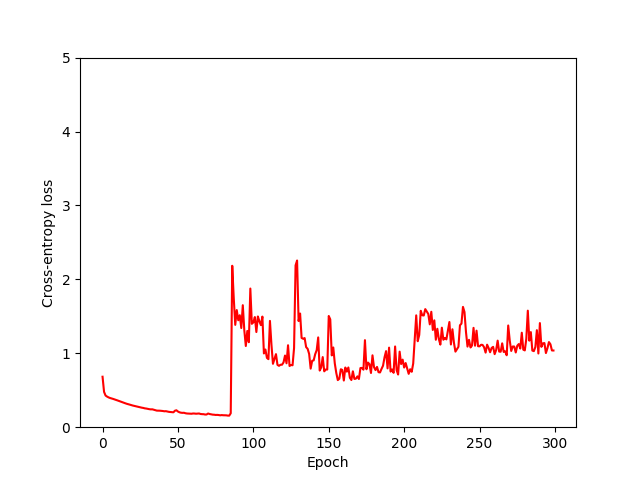
\includegraphics[width=0.8\linewidth]{fig_exp1.png}
\caption{The training cross-entropy loss using the simple model for the NER task.}
\label{fig:fig_exp1}
\end{figure}

% Please add the following required packages to your document preamble:
% 
\begin{table*}[]
\centering
\caption{Results of the Named Entity Recognition experiment. The first four columns are the parameters of each model, and the last two columns are the F-scores on the training data and the development data.}
\label{f1table}
\begin{tabular}{@{}cccc|cc@{}}
\toprule
batch size & learning rate & hidden units & dim\_word\_embed & F-score (train) & F-score (dev) \\ \midrule
16         & 0.1           & 64           & 100              & 1.64             & 1.52           \\
16         & 0.01          & 64           & 100              & 5.36             & 1.58           \\
32         & 0.01          & 64           & 100              & 13.13            & 1.24           \\
32         & 0.01          & 128          & 100              & 17.45            & 5.85           \\
32         & 0.01          & 128          & 200              & 3.44             & 2.63           \\ \bottomrule
\end{tabular}
\end{table*}

\begin{table}[]
\centering
\caption{The precision, recall and F-score of the best model on train data for the NER task. Note that the tags in the table are not completely the same as the labels we use in the experiments. These labels are for evaluation purpose.}
\label{precision}
\begin{tabular}{@{}cccc@{}}
\toprule
Tag            & Precision        & Recall           & F-score       \\ \midrule
LOC              & 37.53\%          & 8.22\%           & 13.49          \\
MISC             & 18.96\%          & 4.18\%           & 6.85           \\
ORG              & 58.32\%          & 23.10\%          & 33.10          \\
PER              & 16.40\%          & 8.95\%           & 11.58          \\ \midrule
\textbf{Overall} & \textbf{33.05\%} & \textbf{11.86\%} & \textbf{17.45} \\ \bottomrule
\end{tabular}
\end{table}



% \begin{table*}
% \renewcommand\thetable{1}
% \begin{center}
% \begin{tabular}{l|c|c|c|c}
% \hline
% Tag & Precision(\%) & Recall(\%) & F-score\\
% \hline\hline
% avg & 80.03 & 33.05 & 11.86 & 17.45 \\
% \hline
% LOC & 37.53 & 8.22 & 13.49 & 1524\\
% MISC & 18.96 & 4.18 & 6.85 & 733 \\
% \hline
% \end{tabular}
% \end{center}
% \caption{NER baseline result}
% \label{tbl:ner_baseline}
% \end{table*}

We also report performance of different parameter settings on train data and development data sets for NER tasks in Table \ref{f1table}. Starting from the basic model, we try several values for each hyper-parameters and report the F1 scores using the official CONLL-2003 evaluation tool \cite{tjongkimsang2003conll}. Table \ref{precision} records the precision, recall and F1 score of the best model found in Table \ref{f1table}. 

% For the CCG SuperTagging task, we perform a preliminary experiment with $batch\_size=32$, $learning\_rate = 0.05$, $dim\_word\_embed =50$, $dim\_label\_embed =10$ and $hidden\_units=64$


%%%%%%%%%%%%%%%%%%%%%%%%%%%%%%%%%
%          DISCUSSION           
%%%%%%%%%%%%%%%%%%%%%%%%%%%%%%%%%
% results 
\section{Discussion} \label{sec:discussion}% of baseline 
% discussion of results 

\subsection{Analysis of the Current Results}

\begin{figure}[t]
\centering
%\fbox{\rule{0pt}{2in} \rule{0.9\linewidth}{0pt}}
   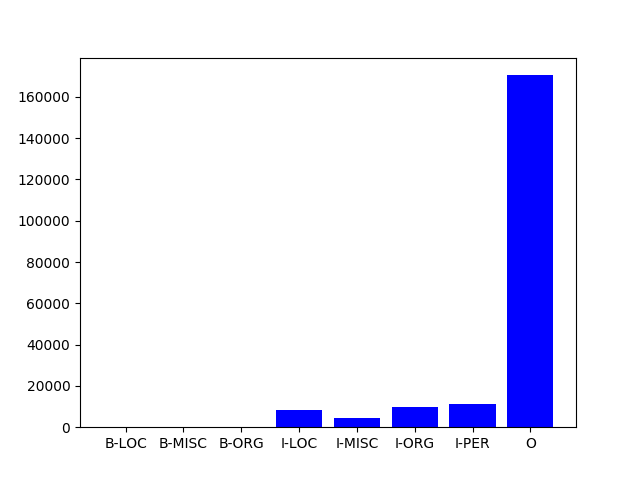
\includegraphics[width=0.8\linewidth]{NER_groundtruths.png}
   \caption{Entity distribution of the CONLL-2003 NER dataset. Tag 'O' is overly dominant.}
\label{fig_ner_gt}
\end{figure}

As seen in Figure~\ref{fig_ner_gt}, the dataset is largely skewed, particularly to the tag 'O', which makes the task hard. Empirically, we find the following trend from Tables \ref{f1table} and \ref{precision}:
\begin{enumerate}
	\item The loss function value decreases faster when using some smaller batch size (we found the batch size of 16 works well). This can be understood by realizing that, with smaller batch size, we perform more updates within one epoch, therefore improving the loss decreasing rate per epoch. However, if the batch size is too small, the training speed will become much slower.
    \item Larger dimension for the hidden state helps. This is expected because with large hidden dimension more context is remembered to be passed from the encoder to the decoder. Since we do not use attention in this assignment, we heavily rely on the hidden state to deliver all the information in the input sequence.
    \item Using smaller learning rate for the SGD can be helpful. In Figure \ref{fig:fig_exp1} we observe that the loss function tends to be unstable at the later epochs of training. We found that by using smaller learning rate we can usually have more epochs that have stable training curve. However, if the learning rate is too small, the training process will also become too slow.
    \item We find in our experiments that using smaller size of word embedding dimension (e.g.~around 100) seems to lead to better performance. At this stage we have not identified the reason for this phenomenon or whether this is really a general trend.
\end{enumerate}




\subsection{Improvement Directions}
\label{ssec:Improvement}

We find that our F-score is much lower than the baseline number shown in \citet{goyal2018continuous}. In addition, from Figure \ref{fig:fig_exp1} we notice that the training loss curve becomes unstable at later epochs. To improve the F-score and the training process, we find many possible directions to pursue:

\begin{enumerate}
	\item \emph{Use bi-directional LSTM for encoder.} We currently only use the single direction LSTM for encoder. To capture the context better, we can use bi-directional LSTM for encoder in the future.
    \item \emph{Add attention mechanism.} In the task such as NER, even if there is only some fixed attention applied, the result is likely to be improved. This is because the named entity type of each word in the input sequence is mostly determined by the word itself (from human experience).
    \item \emph{Add general beam search (not just greedy search).} Currently in test-time decoding we only implemented the greedy search, which is only a special case of the general beam search (with beam size of 1). With adjustable beam size can potentially improve the search results.
    \item \emph{Experiment on different optimizers.} We use the vanilla SGD optimizer in this assignment. Without suitably adjusting the learning rate dynamically, it is likely that our training saturates at some point during the training process, and cannot improve the F-score or accuracy. We can try to dynamically adjust the learning rate or use different optimizers to see whether the training process would improve.
    \item \emph{Be aware of the exploding gradient (or also the vanishing gradient) problem.} We noticed the instability of the training loss curve. We plan to check whether it is caused by the exploding gradient problem.
\end{enumerate}


%%%%%%%%%%%%%%%%%%%%%%%%%%%%%%%%%
%          CONCLUSION           
%%%%%%%%%%%%%%%%%%%%%%%%%%%%%%%%%
\section{Conclusion} \label{sec:conclusion}
In this report we have demonstrated our preliminary seq2seq model with the basic greedy search for decoding phase. For experiment, we have proved our concept through a baseline task of Name Entity Recognition. Along with this task, we have also completed our code for CCG Supertagging, but not yet reported due to lack of time and resources. We plan to reproduce results for both tasks from \citet{goyal2018continuous} in our Assignment 2 report. All the code is now made available in our github repository\footnote{\url{https://github.com/ShuxinLin/nn4nlp_project/}}. 




% \begin{quote}
% \begin{verbatim}
% \usepackage{times}
% \usepackage{latexsym}
% \end{verbatim}
% \end{quote}
% in the preamble. If Times Roman is unavailable, use \textbf{Computer
%   Modern Roman} (\LaTeX2e{}'s default).  Note that the latter is about
%   10\% less dense than Adobe's Times Roman font.

% \begin{table}[t!]
% \begin{center}
% \begin{tabular}{|l|rl|}
% \hline \bf Type of Text & \bf Font Size & \bf Style \\ \hline
% paper title & 15 pt & bold \\
% author names & 12 pt & bold \\
% author affiliation & 12 pt & \\
% the word ``Abstract'' & 12 pt & bold \\
% section titles & 12 pt & bold \\
% subsection titles & 11 pt & bold \\
% document text & 11 pt  &\\
% captions & 11 pt & \\
% abstract text & 11 pt & \\
% bibliography & 10 pt & \\
% footnotes & 9 pt & \\
% \hline
% \end{tabular}
% \end{center}
% \caption{\label{font-table} Font guide. }
% \end{table}


% %Use 11 points for text and subsection headings, 12 points for section headings and 15 points for the title. 


% \begin{table}
% \centering
% \small
% \begin{tabular}{cc}
% \begin{tabular}{|l|l|}
% \hline
% \textbf{Command} & \textbf{Output}\\\hline
% \verb|{\"a}| & {\"a} \\
% \verb|{\^e}| & {\^e} \\
% \verb|{\`i}| & {\`i} \\ 
% \verb|{\.I}| & {\.I} \\ 
% \verb|{\o}| & {\o} \\
% \verb|{\'u}| & {\'u}  \\ 
% \verb|{\aa}| & {\aa}  \\\hline
% \end{tabular} & 
% \begin{tabular}{|l|l|}
% \hline
% \textbf{Command} & \textbf{ Output}\\\hline
% \verb|{\c c}| & {\c c} \\ 
% \verb|{\u g}| & {\u g} \\ 
% \verb|{\l}| & {\l} \\ 
% \verb|{\~n}| & {\~n} \\ 
% \verb|{\H o}| & {\H o} \\ 
% \verb|{\v r}| & {\v r} \\ 
% \verb|{\ss}| & {\ss} \\\hline
% \end{tabular}
% \end{tabular}
% \caption{Example commands for accented characters, to be used in, {\em e.g.}, \BibTeX\ names.}\label{tab:accents}
% \end{table}



% \begin{table*}
% \centering
% \begin{tabular}{lll}
%   output & natbib & previous ACL style files\\
%   \hline
%   \citep{Gusfield:97} & \verb|\citep| & \verb|\cite| \\
%   \citet{Gusfield:97} & \verb|\citet| & \verb|\newcite| \\
%   \citeyearpar{Gusfield:97} & \verb|\citeyearpar| & \verb|\shortcite| \\
% \end{tabular}
% \caption{Citation commands supported by the style file.
%   The citation style is based on the natbib package and
%   supports all natbib citation commands.
%   It also supports commands defined in previous ACL style files
%   for compatibility.
%   }
% \end{table*}



% include your own bib file like this:
%\bibliographystyle{acl}
%\bibliography{acl2018}
\bibliography{acl2018}
\bibliographystyle{acl_natbib}

% \appendix

% \section{Supplemental Material}
% \label{sec:supplemental}
% ACL 2018 also encourages the submission of supplementary material
% to report preprocessing decisions, model parameters, and other details
% necessary for the replication of the experiments reported in the 
% paper. Seemingly small preprocessing decisions can sometimes make
% a large difference in performance, so it is crucial to record such
% decisions to precisely characterize state-of-the-art methods.

% Nonetheless, supplementary material should be supplementary (rather
% than central) to the paper. \textbf{Submissions that misuse the supplementary 
% material may be rejected without review.}
% Essentially, supplementary material may include explanations or details
% of proofs or derivations that do not fit into the paper, lists of
% features or feature templates, sample inputs and outputs for a system,
% pseudo-code or source code, and data. (Source code and data should
% be separate uploads, rather than part of the paper).

% The paper should not rely on the supplementary material: while the paper
% may refer to and cite the supplementary material and the supplementary material will be available to the
% reviewers, they will not be asked to review the
% supplementary material.

% Appendices ({\em i.e.} supplementary material in the form of proofs, tables,
% or pseudo-code) should come after the references, as shown here. Use
% \verb|\appendix| before any appendix section to switch the section
% numbering over to letters.

% \section{Multiple Appendices}
% \dots can be gotten by using more than one section. We hope you won't
% need that.

\end{document}
